\documentclass[12pt]{article}
\usepackage[utf8]{inputenc}
\usepackage{float}
\usepackage{amsmath}
\usepackage{tikz}
\usepackage{tabularx}

\usepackage[hmargin=3cm,vmargin=6.0cm]{geometry}
%\topmargin=0cm
\topmargin=-2cm
\addtolength{\textheight}{6.5cm}
\addtolength{\textwidth}{2.0cm}
%\setlength{\leftmargin}{-5cm}
\setlength{\oddsidemargin}{0.0cm}
\setlength{\evensidemargin}{0.0cm}

%misc libraries goes here



\begin{document}

\section*{Student Information } 
%Write your full name and id number between the colon and newline
%Put one empty space character after colon and before newline
Full Name :  Mehmet Erdeniz Aydoğdu \\
Id Number :  2380103 \\

% Write your answers below the section tags
\section*{Answer 1}
\renewcommand{\labelenumi}{\textbf{\alph{enumi}.}}
\begin{enumerate}
    \item The Hasse Diagram for POSET: \newline
    \begin{center}
    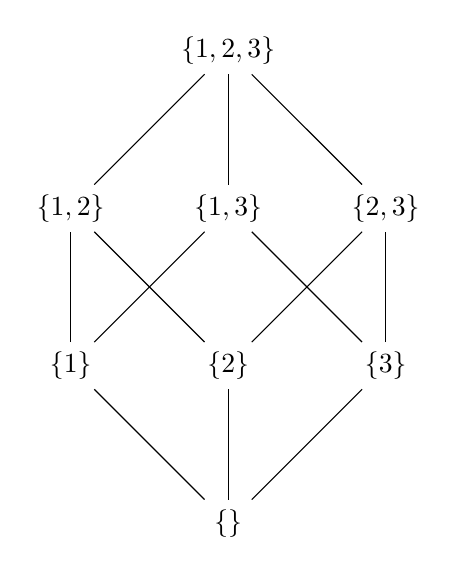
\begin{tikzpicture}
    \node (mid) at (0,0) {$\{1,3\}$};
    \node (top) at (0,2) {$\{1,2,3\}$};
    \node (left1) at (-2,0)  {$\{1,2\}$};
    \node (right1) at (2,0) {$\{2,3\}$};
    \node (mid2) at (0,-2) {$\{2\}$};
    \node (left2) at (-2,-2) {$\{1\}$};
    \node (right2) at (2,-2) {$\{3\}$};
    \node (bottom) at (0,-4) {$\{\}$};
    \draw (mid) -- (top);
    \draw (left1) -- (top);
    \draw (right1) -- (top);
    \draw (left2) -- (mid);
    \draw (right2) -- (mid);
    \draw (mid2) -- (left1);
    \draw (mid2) -- (right1);
    \draw (left2) -- (left1);
    \draw (right2) -- (right1);
    \draw (bottom) -- (left2);
    \draw (bottom) -- (mid2);
    \draw (bottom) -- (right2);
\end{tikzpicture}
\end{center}
    \item For each subset $B$ and $C$ of $A$, since the least upper bound of $B$ and $C$ is $B \cup C$ and the greatest lower bound of $B$ and $C$ is $B \cap C$, it is a lattice.
    \item $\{1,2,3\}$ is the maximal element because there is no element $x \in P(A)$ such that $\{1,2,3\} \subseteq x$
    \item $\{\}$ is the minimal element because there is no element $x \in P(A)$ such that $x \subseteq \{\}$.
    \item For all $x \in P(A)$, $x \subseteq \{1,2,3\}$, thus, $\{1,2,3\}$ is the greatest element.
    \item For all $x \in P(A)$, $\{\} \subseteq x$, thus, $\{\}$ is the least element.
    \item Upper bounds of $\{1\}$ and $\{3\}$ are $\{1,3\}$ and $\{1,2,3\}$. Since $\{1,3\} \subseteq \{1,2,3\}$, $\{1,3\}$ is the least upper bound of $\{1\}$ and $\{3\}$.
\end{enumerate}
\newpage
\section*{Answer 2}
\renewcommand{\labelenumi}{\textbf{\alph{enumi}.}}
\begin{enumerate}
    \item deg(a) = 2, deg(b) = 4, deg(c) = 2, deg(d) = 3 and deg(e) = 3. Thus, sum of degrees of all nodes is 2+4+2+3+3 = 14.
    \item If we order the vertices as a, b, c, d, e; the adjacency matrix representation of G is:
    \begin{center}
    $\begin{bmatrix}
    0 & 1 & 0 & 0 & 1\\
    1 & 0 & 1 & 1 & 1\\
    0 & 1 & 0 & 1 & 0\\
    0 & 1 & 1 & 0 & 1\\
    1 & 1 & 0 & 1 & 0
    \end{bmatrix}$
    \end{center}
    Thus, 14 is the number of non-zero entries.
    \item There are 7 edges and 5 vertices. We order the columns $e_1, e_2, e_3, e_4, e_5, e_6, e_7$ and rows a, b, c, d, e. Then, the incident matrix representation of G is:
    \begin{center}
        $\begin{bmatrix}
        1 & 0 & 0 & 0 & 1 & 0 & 0\\
        1 & 1 & 0 & 0 & 0 & 1 & 1\\
        0 & 1 & 1 & 0 & 0 & 0 & 0\\
        0 & 0 & 1 & 1 & 0 & 1 & 0\\
        0 & 0 & 0 & 1 & 1 & 0 & 1
        \end{bmatrix}$
    \end{center}
    Thus, 14 is the number of non-zero entries.
    \item Yes, it has.
    \begin{center}
    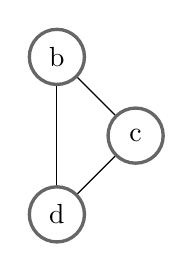
\begin{tikzpicture}[round/.style={circle, draw=black!60, very thick, minimum size=7mm}]
    \node [round](b) at (0,0) {b};
    \node [round](d) at (0,-2) {d};
    \node [round](c) at (1,-1) {c};
    \draw (b) -- (d);
    \draw (b) -- (c);
    \draw (c) -- (d);
    \end{tikzpicture}
    \end{center}
    \item G is not bipartite. If we remove the edges between (a,b), (b,c) and (d,e), the subgraph is a bipartite graph such that: 
    \begin{center}
        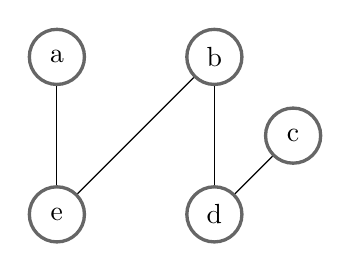
\begin{tikzpicture}[round/.style={circle, draw=black!60, very thick, minimum size=7mm}]
        \node [round] (a) at (0,0) {a};
        \node [round] (b) at (2,0) {b};
        \node [round] (e) at (0,-2) {e};
        \node [round] (d) at (2,-2) {d};
        \node [round] (c) at (3,-1) {c};
        \draw (a) -- (e);
        \draw (b) -- (e);
        \draw (d) -- (b);
        \draw (c) -- (d);
        \end{tikzpicture}
    \end{center}
    \item Every edge in G can have two directions in a directed graph. Thus, the number of directed graphs is $2\times2\times2\times2\times2\times2\times2 = 2^7$
    \item 
    \item Number of connected components of G is 1 because G is a connected graph.
    \item The condition for a graph to have an Euler circuit, all vertices have to have even degrees. As deg(e) = 3 and deg(d) = 3; G doesn't have an Euler circuit.
    \item As stated in (i), G doesn't have an Euler circuit but it has exactly two vertices of odd degree. Thus, it has an Euler path, which is: e, a, b, c, d, b, e, d.
    \item It has more than one Hamilton circuit. One of them is: a,b,c,d,e,a.
    \item It has more than one Hamilton circuit. One of them is between a and e: a,b,c,d,e.
\end{enumerate}

\section*{Answer 3}
Adjacency matrix of G is:
    \begin{center}
        $\bordermatrix{~ & a & b & c & d & e & f & g & h \cr 
        a & 0 & 1 & 0 & 1 & 1 & 1 & 0 & 0 \cr
        b & 1 & 0 & 1 & 0 & 1 & 0 & 1 & 0 \cr
        c & 0 & 1 & 0 & 1 & 0 & 0 & 1 & 1 \cr
        d & 1 & 0 & 1 & 0 & 0 & 1 & 0 & 1 \cr
        e & 1 & 1 & 0 & 0 & 0 & 1 & 0 & 1 \cr
        f & 1 & 0 & 0 & 1 & 1 & 0 & 1 & 0 \cr
        g & 0 & 1 & 1 & 0 & 0 & 1 & 0 & 1 \cr
        h & 0 & 0 & 1 & 1 & 1 & 0 & 1 & 0 \cr
        }$
    \end{center}
    And, if we order vertices as a', c', e', g', b', h', d', f'; adjacency matrix of H is:
    \begin{center}
        $\bordermatrix{~ & a' & c' & e' & g' & b' & h' & d' & f' \cr 
        a' & 0 & 1 & 0 & 1 & 1 & 1 & 0 & 0 \cr
        c' & 1 & 0 & 1 & 0 & 1 & 0 & 1 & 0 \cr
        e' & 0 & 1 & 0 & 1 & 0 & 0 & 1 & 1 \cr
        g' & 1 & 0 & 1 & 0 & 0 & 1 & 0 & 1 \cr
        b' & 1 & 1 & 0 & 0 & 0 & 1 & 0 & 1 \cr
        h' & 1 & 0 & 0 & 1 & 1 & 0 & 1 & 0 \cr
        d' & 0 & 1 & 1 & 0 & 0 & 1 & 0 & 1 \cr
        f' & 0 & 0 & 1 & 1 & 1 & 0 & 1 & 0 \cr
        }$
    \end{center}
    Then, there exist one-to-one correspondence between G and H. Thus, G and H are isomorphic.

\section*{Answer 4}

\begin{tabularx}{0.4\textwidth} { 
  | >{\raggedright\arraybackslash}X 
  | >{\centering\arraybackslash}X 
  | >{\raggedleft\arraybackslash}X | }
 \hline
 Vertice & Distance & Path \\
 \hline
 a*  & 0  & -  \\
\hline
 b  & 3  & a,b  \\
\hline
 h  & 4  & a,h  \\
\hline
 e  & 5  & a,e  \\
\hline
\end{tabularx}
\newline \newline
Start with a. (Other nodes with $\infty$ distance are not included due to spacing.)\newline\newline
\begin{tabularx}{0.4\textwidth} { 
  | >{\raggedright\arraybackslash}X 
  | >{\centering\arraybackslash}X 
  | >{\raggedleft\arraybackslash}X | }
 \hline
 Vertice & Distance & Path \\
 \hline
 a*  & 0  & a  \\
\hline
 b*  & 3  & a,b  \\
\hline
 h  & 4  & a,h  \\
\hline
 e  & 5  & a,e  \\
\hline
 c  & 5  & a,b,c  \\
\hline
 f  & 10  & a,b,f  \\
\hline
\end{tabularx}
\newline \newline
Proceed with the vertice with the shortest distance, which is b. 
\newline\newline
\begin{tabularx}{0.4\textwidth} { 
  | >{\raggedright\arraybackslash}X 
  | >{\centering\arraybackslash}X 
  | >{\raggedleft\arraybackslash}X | }
 \hline
 Vertice & Distance & Path \\
 \hline
 a*  & 0  & a  \\
\hline
 b*  & 3  & a,b  \\
\hline
 h*  & 4  & a,h  \\
\hline
 e  & 5  & a,e  \\
\hline
 c  & 5  & a,b,c  \\
\hline
 f  & 9  & a,h,f  \\
\hline
 i  & 6  & a,h,i  \\
\hline
\end{tabularx}
\newline \newline
Next vertice is h. Here, path $\{$a,b,f$\}$ is replaced by shorter path $\{$a,h,f$\}$.
\newline\newline
\begin{tabularx}{0.4\textwidth} { 
  | >{\raggedright\arraybackslash}X 
  | >{\centering\arraybackslash}X 
  | >{\raggedleft\arraybackslash}X | }
 \hline
 Vertice & Distance & Path \\
 \hline
 a*  & 0  & a  \\
\hline
 b*  & 3  & a,b  \\
\hline
 h*  & 4  & a,h  \\
\hline
 e*  & 5  & a,e  \\
\hline
 c*  & 5  & a,b,c  \\
\hline
 f  & 7  & a,b,c,f  \\
\hline
 i  & 6  & a,h,i  \\
\hline
 d  & 8  & a,b,c,d  \\
\hline
\end{tabularx}
\newline \newline
Vertice e does not change any shortest path. After e, next vertice is c and here, path $\{$a,h,f$\}$ is replaced by shorter path $\{$a,b,c,f$\}$
\newline\newline
\newpage
\begin{tabularx}{0.4\textwidth} { 
  | >{\raggedright\arraybackslash}X 
  | >{\centering\arraybackslash}X 
  | >{\raggedleft\arraybackslash}X | }
 \hline
 Vertice & Distance & Path \\
 \hline
 a*  & 0  & a  \\
\hline
 b*  & 3  & a,b  \\
\hline
 h*  & 4  & a,h  \\
\hline
 e*  & 5  & a,e  \\
\hline
 c*  & 5  & a,b,c  \\
\hline
 f  & 7  & a,b,c,f  \\
\hline
 i*  & 6  & a,h,i  \\
\hline
 d  & 8  & a,b,c,d  \\
\hline
 j  & 12  & a,h,i,j  \\
\hline
\end{tabularx}
\newline \newline
Proceeding with i. 
\newline\newline
\begin{tabularx}{0.4\textwidth} { 
  | >{\raggedright\arraybackslash}X 
  | >{\centering\arraybackslash}X 
  | >{\raggedleft\arraybackslash}X | }
 \hline
 Vertice & Distance & Path \\
 \hline
 a*  & 0  & a  \\
\hline
 b*  & 3  & a,b  \\
\hline
 h*  & 4  & a,h  \\
\hline
 e*  & 5  & a,e  \\
\hline
 c*  & 5  & a,b,c  \\
\hline
 f*  & 7  & a,b,c,f  \\
\hline
 i*  & 6  & a,h,i  \\
\hline
 d  & 8  & a,b,c,d  \\
\hline
 j  & 12  & a,h,i,j  \\
\hline
 g  & 12  & a,b,c,f,g  \\
\hline
\end{tabularx}
\newline \newline
Proceeding with f. 
\newline\newline
\begin{tabularx}{0.4\textwidth} { 
  | >{\raggedright\arraybackslash}X 
  | >{\centering\arraybackslash}X 
  | >{\raggedleft\arraybackslash}X | }
 \hline
 Vertice & Distance & Path \\
 \hline
 a*  & 0  & a  \\
\hline
 b*  & 3  & a,b  \\
\hline
 h*  & 4  & a,h  \\
\hline
 e*  & 5  & a,e  \\
\hline
 c*  & 5  & a,b,c  \\
\hline
 f*  & 7  & a,b,c,f  \\
\hline
 i*  & 6  & a,h,i  \\
\hline
 d*  & 8  & a,b,c,d  \\
\hline
 j  & 12  & a,h,i,j  \\
\hline
 g  & 12  & a,b,c,f,g  \\
\hline
 k  & 10  & a,b,c,d,k  \\
\hline
\end{tabularx}
\newline \newline
Proceeding with d. 
\newline\newline
\begin{tabularx}{0.4\textwidth} { 
  | >{\raggedright\arraybackslash}X 
  | >{\centering\arraybackslash}X 
  | >{\raggedleft\arraybackslash}X | }
 \hline
 Vertice & Distance & Path \\
 \hline
 a*  & 0  & a  \\
\hline
 b*  & 3  & a,b  \\
\hline
 h*  & 4  & a,h  \\
\hline
 e*  & 5  & a,e  \\
\hline
 c*  & 5  & a,b,c  \\
\hline
 f*  & 7  & a,b,c,f  \\
\hline
 i*  & 6  & a,h,i  \\
\hline
 d*  & 8  & a,b,c,d  \\
\hline
 j*  & 12  & a,h,i,j  \\
\hline
 g*  & 12  & a,b,c,f,g  \\
\hline
 k*  & 10  & a,b,c,d,k  \\
\hline
\end{tabularx}
\newline \newline
Here, we will firstly proceed with k, then j, then g. None of the paths will change. 
\newline \newline
Last table shows us all of the shortest paths starting with a. Thus, shortest path from a to j is $\{$a,h,i,j$\}$ with 12.
\section*{Answer 5}
\renewcommand{\labelenumi}{\textbf{\alph{enumi}.}}
\begin{enumerate}
    \item Using Prim's Algorithm: \newline \newline
        \begin{tabularx}{0.4\textwidth} { 
          | >{\raggedright\arraybackslash}X 
          | >{\centering\arraybackslash}X 
          | >{\raggedleft\arraybackslash}X | }
         \hline
         Choice & Edge & Weight \\
         \hline
         1  & (a,b)  & 1  \\
        \hline
         2  & (d,a)  & 3  \\
        \hline
         3  & (b,c)  & 4  \\
        \hline
         4  & (c,e)  & 2  \\
        \hline
         5  & (c,f)  & 2  \\
        \hline
        \end{tabularx}
    \item Minimum spanning tree: \newline
    \begin{center}
    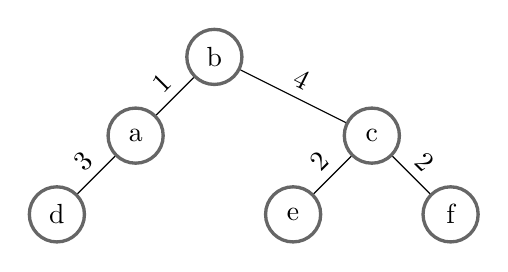
\begin{tikzpicture}[round/.style={circle, draw=black!60, very thick, minimum size=7mm}]
    \node [round](b) at (0,0) {b};
    \node [round](c) at (2,-1) {c};
    \node [round](e) at (1,-2) {e};
    \node [round](f) at (3,-2) {f};
    \node [round](a) at (-1,-1) {a};
    \node [round](d) at (-2,-2) {d};
    \draw  (a) -- (b) node [midway, above, sloped] (TextNode) {1};
    \draw  (a) -- (d) node [midway, above, sloped] (TextNode) {3};
    \draw  (c) -- (b) node [midway, above, sloped] (TextNode) {4};
    \draw  (c) -- (e) node [midway, above, sloped] (TextNode) {2};
    \draw  (c) -- (f) node [midway, above, sloped] (TextNode) {2};
    
\end{tikzpicture}
\end{center}
    \item Because there are edges with equal weights, minimum spanning tree is not unique.
\end{enumerate}

\newpage
\section*{Answer 6}
\renewcommand{\labelenumi}{\textbf{\alph{enumi}.}}
\begin{enumerate}
    \item Number of vertices is 13, number of edges is 12 and the height is 4.
    \item w,s,m,t,q,x,n,y,u,z,v,r,p
    \item s,w,q,m,t,p,x,u,n,y,r,v,z
    \item p,q,s,w,t,m,r,u,x,y,n,v,z
    \item $T$ is not a binary tree. A full $m$-ary tree with $i$ internal vertices contains $n = mi + 1$ vertices. $T$ has 7 internal vertices, which means $n = 2 \times 7 + 1 = 15$. However, $T$ has 13 vertices.
\end{enumerate}

\end{document}